\chapter{Probléma definíció}
Az előző fejezetben bemutatott throughput maximalizálás esetében kikötés volt, hogy minden termék batch mérete rögzített legyen, azaz a termékek batch-jének jövedelmét ismerjük.
Abban az esetben minden taszkhoz egy berendezés hozzárendelése megengedett, azaz csak egy berendezés végezheti el.
Azonban számos esettanulmány és irodalmi példa esetében a batch méretek nem rögzítettek.
Ha több berendezés képes elvégezni ugyanazt a taszkot, akkor ezt megtehetik párhuzamosan.
Ilyen eset főleg a throughput maximalizálás során léphet fel, de megjelenhet makespan minimalizálásnál is.
Az időfelosztásos módszerek meg tudják oldani az ilyen problémákat, azonban az S-gráf keretrendszer esetén néhány módosítás szükséges.
A throughput maximalizálás algoritmusa megköveteli, hogy a recept rögzített, valamint egy termék batch-jének jövedelme is előre ismert legyen.
Az előbb említett problémák esetén viszont egyik sem garantált. 
A javasolt megközelítés szemléltetésére a Kondili és munkatársaitól származó példát veszem igénybe \cite{kondili}.
Ez látható \ref{kondiliPelda} ábrán.

A folyamat 5 taszkból áll: fűtésből, 3 darab reakcióból, és az szétválasztásból.
Ezekhez 4 berendezés áll rendelkezésre: a fűtőtest és szeparátor, mindkettő 100 kilogrammos kapacitással a fűtés és elválasztás folyamatához.
A három reakciós folyamathoz van 2 darab reaktor ugyanakkora feldolgozási idővel.
A kapacitásuk eltér, egyiké 80 kilogramm a másiké pedig 50 kilogramm, de ezeket a reaktorokat párhuzamosan is igénybe lehet venni.
Feltételezzük, hogy az összes egység képes a kapacitásuknál kisebb terheléssel működni, azaz nincs meghatározva, hogy minimálisan mekkora mennyiség szükséges.
A folyamat során két termék készül azonos profittal.
A következő korlátozások fennállnak: nem marad semmilyen köztes anyag a termelő folyamat végén, nem lehet csak az egyes számú terméket gyártani, illetve nincs tárolásra lehetőség a folyamat során.
\begin{figure}[H]
\begin{center}
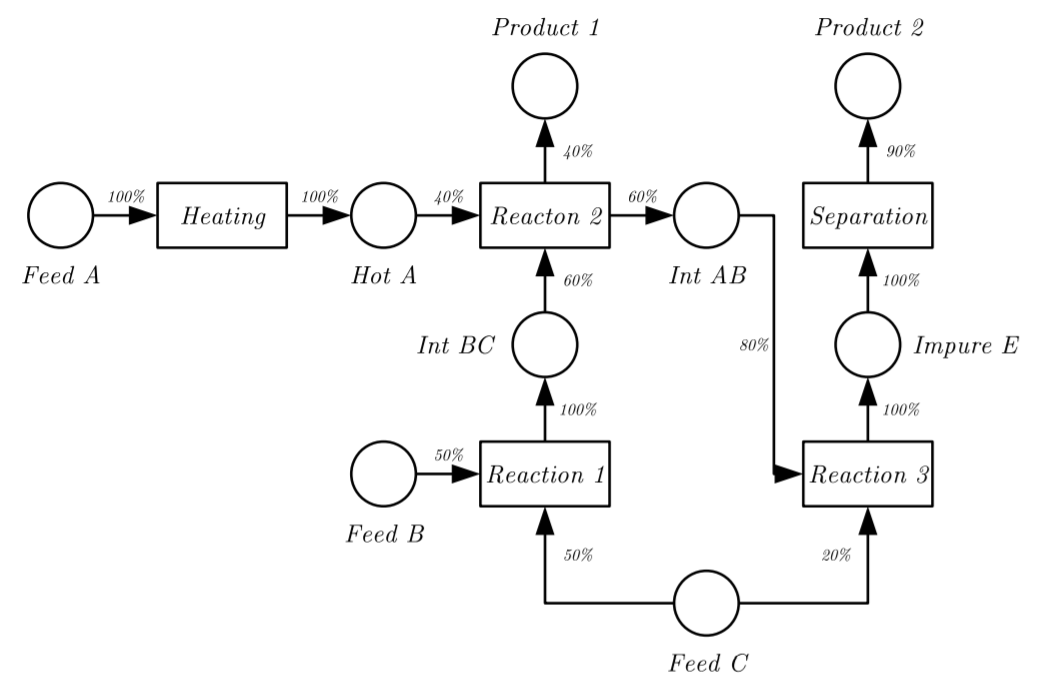
\includegraphics[scale=0.65]{kondiliPelda}
\caption{Kondili példafeladata}
\label{kondiliPelda}
\end{center}
\end{figure}

Mindegyik reakció elvégezhető az egyik, a másik, vagy egyszerre mindkettő reaktor által párhuzamosan.
Ez $3^3 = 27$ rögzített receptet eredményez, amelyek különböző batch mérettel rendelkezhetnek.
Mindegyik esetben különálló S-gráf receptet kell létrehozni, hogy a korábban említett S-gráf algoritmust igénybe lehessen venni profit maximalizálásra, így a legfelső szinten lévő keresési terület 27 dimenziós térré válna.
Ez óriási CPU igényhez vezetne az optimalizálás során, ezért az esetek számának csökkentése elengedhetetlen.

Ha megnézzük a \ref{tabla1} táblázatot, észrevehető, hogy csupán néhány érték ismétlődik.
Ennek oka az anyagok egyensúlyából származik.
Például, hogy ha mind az R1-et mind az R2-t hozzárendeljük a hármas számú reakcióhoz ahelyett, hogy csak az R1 lenne hozzárendelve, akkor sem lesz nagyobb a kimenet, mert a korábbi reakciókból származó pótlás nem éri el a szükséges szintet.
Ha a két különböző eset, $c$ és $c'$, ugyanakkora maximális jövedelemmel rendelkezik, de a $c$ eset csak kisebb részét használja a $c'$ által használt egységeknek, ekkor azt mondjuk, hogy a $c$ \textit{dominálja} a $c'$-t.
A példából látható, hogy a 9-es eset dominálja a 27-es esetet.
Továbbá a 24-es eset dominálva van a 4, 5, 6, 13, 14, 15, 22, 23 esetek által.
Megállapíthatjuk, hogy ha egy eset legalább egy másik által dominálva van, akkor azt kizárhatjuk a vizsgálatból, mert az továbbra is garantálva van, hogy megtalálja az optimális megoldást.
A \ref{tabla3} táblázat tartalmazza azokat az eseteket, amelyek nincsenek dominálva más esetek által. 

\begin{table}
	\begin{center}
		\caption{A 27 rögzített recept Kondili példájához}
		\captionsetup[table]{skip=10pt}
		\label{tabla1}
		\begin{tabular}{r|ccc|l}
		Eset & Reakció 1 & Reakció 2 & Reakció 3 & Max bevétel  \\ 
		\hline
		1    & R1        & R1        & R1        & 86,00        \\
		2    & R1        & R1        & R2        & 71,67        \\
		3    & R1        & R1        & R1\&R2    & 86,00        \\
		4    & R1        & R2        & R1        & 53,75        \\
		5    & R1        & R2        & R2        & 53,75        \\
		6    & R1        & R2        & R1\&R2    & 53,75        \\
		7    & R1        & R1\&R2    & R1        & 114,76       \\
		8    & R1        & R1\&R2    & R2        & 71,67        \\
		9    & R1        & R1\&R2    & R1\&R2    & 139,75       \\
		10   & R2        & R1        & R1        & 86,00        \\
		11   & R2        & R1        & R2        & 71,67        \\
		12   & R2        & R1        & R1\&R2    & 86,00        \\
		13   & R2        & R2        & R1        & 53,75        \\
		14   & R2        & R2        & R2        & 53,75        \\
		15   & R2        & R2        & R1\&R2    & 53,75        \\
		16   & R2        & R1\&R2    & R1        & 89,58        \\
		17   & R2        & R1\&R2    & R2        & 71,67        \\
		18   & R2        & R1\&R2    & R1\&R2    & 89,58        \\
		19   & R1\&R2    & R1        & R1        & 86,00        \\
		20   & R1\&R2    & R1        & R2        & 71,67        \\
		21   & R1\&R2    & R1        & R1\&R2    & 86,00        \\
		22   & R1\&R2    & R2        & R1        & 53,75        \\
		23   & R1\&R2    & R2        & R2        & 53,75        \\
		24   & R1\&R2    & R2        & R1\&R2    & 53,75        \\
		25   & R1\&R2    & R1\&R2    & R1        & 114,76       \\
		26   & R1\&R2    & R1\&R2    & R2        & 71,67        \\
		27   & R1\&R2    & R1\&R2    & R1\&R2    & 139,75      
		\end{tabular}
	\end{center}
\end{table}

	

\begin{table}[H]
	\begin{center}
		\caption{Nem dominált esetek bevétel szerint növekvő sorrendben}
		\captionsetup[table]{skip=10pt}	
		\label{tabla2}	
		\begin{tabular}{r|ccc|l}
		Eset & Reakció 1 & Reakció 2 & Reakció 3 & Max bevétel  \\ 
		\hline
		4    & R1        & R2        & R1        & 53,75        \\
		5    & R1        & R2        & R2        & 53,75        \\
		13   & R2        & R2        & R1        & 53,75        \\
		14   & R2        & R2        & R2        & 53,75        \\
		2    & R1        & R1        & R2        & 71,67        \\
		11   & R2        & R1        & R2        & 71,67        \\
		1    & R1        & R1        & R1        & 86,00        \\
		10   & R2        & R1        & R1        & 86,00        \\
		16   & R2        & R1\&R2    & R1        & 89,58        \\
		7    & R1        & R1\&R2    & R1        & 114,67       \\
		9    & R1        & R1\&R2    & R1\&R2    & 139,75      
		\end{tabular}
	\end{center}
\end{table}

Ezután az esetszám csökkenés után is még mindig 11 esetet kellene az S-gráf algoritmusnak megvizsgálni.
Annak érdekében, hogy tovább csökkenjen ez a szám több esetet is össze lehet vonni.
Például a 4-es és 5-ös eset teljes mértékben megegyezik, azzal a kivétellel, hogy a harmadik reakciós folyamatot más reaktor végzi.
Ezt a két esetet össze lehet vonni úgy, hogy a harmadik reakciónál R1 vagy R2-es reaktor ($R1 \vee R2$) üzemel.
A \ref{tabla3} táblázatban látható a végleges összevonás eredménye.

\begin{table}[H]
	\begin{center}
		\caption{Összevont, nem dominált esetek bevétel szerint növekvő sorrendben}
		\captionsetup[table]{skip=10pt}	
		\label{tabla3}	
		\begin{tabular}{r|ccc|l}
		Eset      & Reakció 1~ & Reakció 2 & Reakció 3 & Max bevétel  \\ 
		\hline
		4,5,13,14 & $R1 \vee R2$      & R2 & $R1 \vee R2$     & 53,75        \\
		2,11      & $R1 \vee R2$      & R1        & R2        & 71,67        \\
		1,10      & $R1 \vee R2$      & R1        & R1        & 86,00        \\
		16        & R2         & R1\&R2    & R1        & 89,58        \\
		7         & R1         & R1\&R2    & R1        & 114,67       \\
		9         & R1         & R1\&R2    & R1\&R2    & 139,75      
		\end{tabular}
	\end{center}
\end{table}

Látható, hogy az ilyen típusú feladatoknál nem lehet közvetlenül a megoldó programot igénybe venni a feladat megoldásához, szükség van előzetes lépésekre, hogy megfelelő formába kerüljön a feladat.
Ez mindig plusz időbe kerül, és ez az idő annál nagyobb lehet, minél több taszk és berendezés szerepel az adott feladatban.
A következő fejezetben bemutatott új módszer esetén ezek a lépések elhagyhatóak, ezáltal időt lehet megspórolni.